\chapter{Gas Species and Smoke}

CFAST simulates a fire as a mass of fuel that burns at a prescribed rate and releases both energy and combustion products.  CFAST calculates species production based on these user-defined production yields, and both the mass burning rate and the resulting energy and species generation may be limited by the oxygen available for combustion.  Mass and species concentrations, assumed to be homogeneous throughout each layer, are tracked by the model as gases flow through openings in a structure to other compartments in the structure or to the outdoors.

The fire chemistry scheme in CFAST is essentially a species balance from user-prescribed species yields and the oxygen available for combustion.  For a given scenario, the user specifies the fuel that is burned, and the yield of CO and soot. Once generated, it is a matter of bookkeeping to track the mass of species throughout the various control volumes in a simulated building.  It does, however, provide a check of the flow algorithms within the model. Since the major species (CO and CO$_2$) are generated only by the fire, the relative accuracy of the predicted values throughout multiple rooms of a structure should be comparable.

Gas sampling data are available from a number of the experimental tests. Species yields for CFAST simulations were taken from the experimental reports.

\section{Oxygen, CO$_2$, and CO}

Generation of oxygen and CO$_2$ are calculated by CFAST based on the user-specified fuel and a simple combustion reaction. CFAST treats CO like all other combustion products, with an overall mass balance dependent on interrelated user-specified species yields for major combustion species. To model CO, the user prescribes the CO yield relative to the mass burning rate. Details are available in the CFAST Technical Reference Guide \cite{CFAST_Tech_Guide_7}.  

Figure \ref{fig:Species_Scatter} shows a comparison of predicted and measured values for oxygen and carbon dioxide concentrations, along with a summary of the relative difference for the tests.
\label{Oxygen Concentration}
\label{Carbon Dioxide Concentration}
\label{Carbon Monoxide Concentration}

\begin{figure}
\begin{tabular*}{\textwidth}{l@{\extracolsep{\fill}}r}
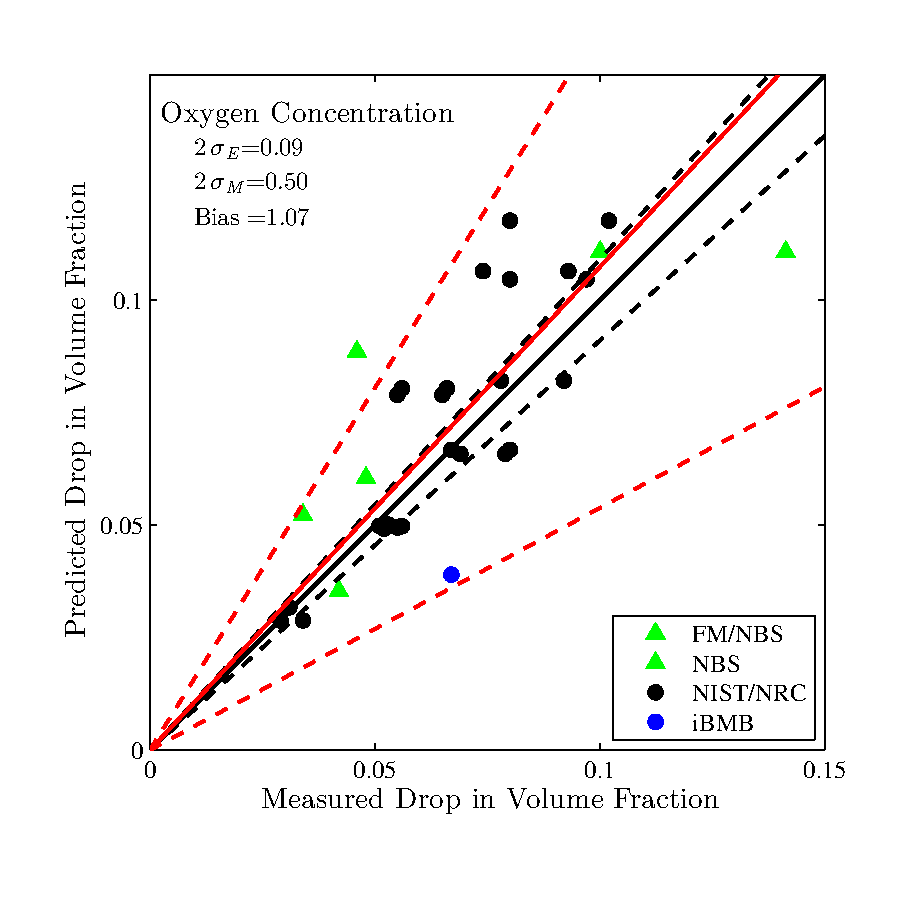
\includegraphics[width=3.0in]{SCRIPT_FIGURES/ScatterPlots/Oxygen_Concentration} &
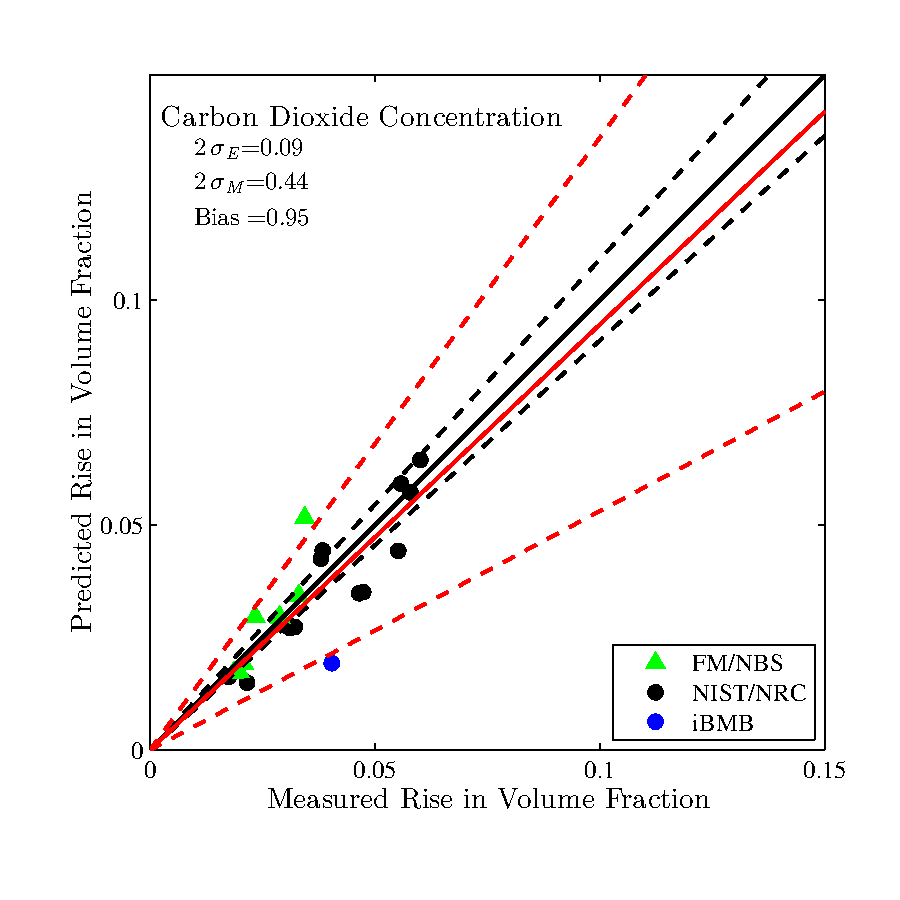
\includegraphics[width=3.0in]{SCRIPT_FIGURES/ScatterPlots/Carbon_Dioxide_Concentration} \\
\multicolumn{2}{c}{\includegraphics[width=3.0in]{SCRIPT_FIGURES/ScatterPlots/Carbon_Monoxide_Concentration}} \\
\end{tabular*}
\caption{Comparison of Measured and Predicted Oxygen Concentration, Carbon Dioxide Concentration, and Carbon Monoxide Concentration.} \label{fig:Species_Scatter}
\end{figure}


\section{Smoke}

CFAST treats smoke like all other combustion products, with an overall mass balance dependent on interrelated user-specified species yields for major combustion species.  To model smoke, the user prescribes the smoke yield relative to the mass burning rate.  A simple combustion chemistry scheme in the model then determines the smoke particulate concentration in the form of an optical density.  Figure \ref{fig:Smoke_Scatter} shows a comparison of predicted and measured values for smoke concentration along with a summary of the relative difference for the tests.
\label{Smoke Concentration}

\begin{figure}
\begin{center}
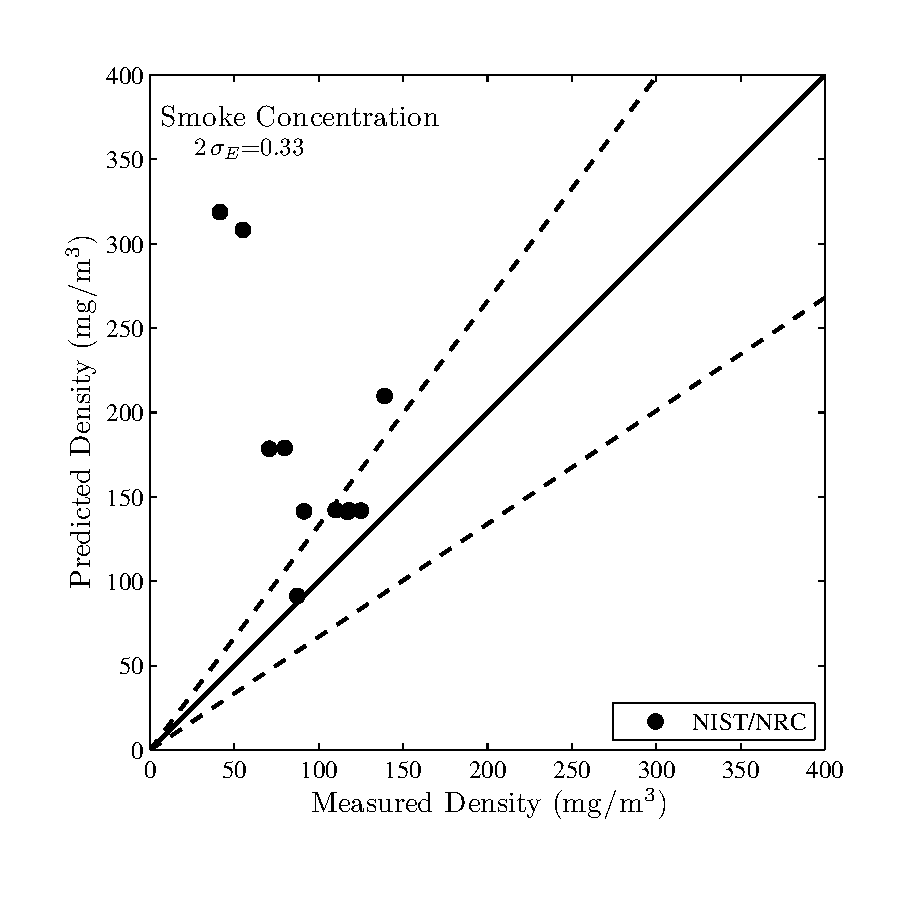
\includegraphics[width=4.0in]{SCRIPT_FIGURES/ScatterPlots/Smoke_Concentration}
\end{center}
\caption{Comparison of Measured and Predicted Smoke Concentration.} \label{fig:Smoke_Scatter}
\end{figure}
